\documentclass[11pt,a4paper,BCOR12mm, headexclude, footexclude, twoside, openright]{scrartcl} 
\usepackage[scaled]{helvet}
\usepackage[british]{babel}
\usepackage[utf8]{inputenc}
\usepackage[T1]{fontenc}
\usepackage{fancyhdr}
\usepackage{lastpage}
\usepackage{ifthen}
\usepackage{amsmath,amsfonts,amsthm}
\usepackage{sfmath}
\usepackage{makecell}
\usepackage{booktabs}
\usepackage{sectsty}
\usepackage{xcolor}
\usepackage{tikz}
%\KOMAoptions{optionenliste}
%\KOMAoptions{Option}{Werteliste}

\newcommand*{\TakeFourierOrnament}[1]{{%
\fontencoding{U}\fontfamily{futs}\selectfont\char#1}}
\newcommand*{\danger}{\TakeFourierOrnament{66}}
\addtokomafont{caption}{\small}
%\setkomafont{descriptionlabel}{\normalfont
%	\bfseries}
\setkomafont{captionlabel}{\normalfont
	\bfseries}
\let\oldtabular\tabular
\renewcommand{\tabular}{\sffamily\oldtabular}
\KOMAoptions{abstract=true}
%\setkomafont{footnote}{\sffamily}
%\KOMAoptions{twoside=true}
%\KOMAoptions{headsepline=true}
%\KOMAoptions{footsepline=true}
\renewcommand\familydefault{\sfdefault}
\renewcommand{\arraystretch}{1.1}
\newcommand{\horrule}[1]{\rule{\linewidth}{#1}}
\setlength{\textheight}{230mm}
\allsectionsfont{\centering \normalfont\scshape}
\let\tmp\oddsidemargin
\let\oddsidemargin\evensidemargin
\let\evensidemargin\tmp
\reversemarginpar

\numberwithin{equation}{section} % Number equations within sections (i.e. 1.1, 1.2, 2.1, 2.2 instead of 1, 2, 3, 4)
\numberwithin{figure}{section} % Number figures within sections (i.e. 1.1, 1.2, 2.1, 2.2 instead of 1, 2, 3, 4)
\numberwithin{table}{section} % Number tables within sections (i.e. 1.1, 1.2, 2.1, 2.2 instead of 1, 2, 3, 4)

\setlength\parindent{0pt}

\definecolor{CFFFFFF}{HTML}{FFFFFF}
\definecolor{C000000}{HTML}{000000}
\definecolor{CFF0000}{HTML}{FF0000}
\begin{document}

\tikzstyle{shador} = [circle,shading=axis, left color=green, right color=red,
    minimum size=1cm]

%\sffamily
\fancypagestyle{plain}
{%
  \renewcommand{\headrulewidth}{0pt}%
  \renewcommand{\footrulewidth}{0.5pt}
  \fancyhf{}%
  \fancyfoot[R]{\emph{\footnotesize Page \thepage\ of \pageref{LastPage}}}%
  \fancyfoot[C]{\emph{\footnotesize Samy Aittahar}}%
}

\thispagestyle{plain}

\titlehead
{
	University of Liège\hfill
    INFO8006%
}
\subject{\vspace{-1ex} \horrule{2pt}\\[0.15cm] {\textsc{\texttt{Introduction to AI}}}}
\title{Assignment 2}
\subtitle{\textsc{\texttt{When AI play games}}\\\horrule{2pt}\\[0.5cm]}
\author{\bfseries{Samy Aittahar}\vspace{-2ex}}
\date{\begin{tabular}{cc}
  \textsc{Date:}& \textsc{\emph{\today}}
\end{tabular}}
\maketitle

%\begin{abstract}
%\end{abstract}

%--------------------------------------------

\section{Connect three}


Let us consider the game grid below as a variant of the connect-four game. Each player has 8 tokens of its own color (green or red). A token can be inserted in a non-fully filled column and fall in the deepest free node in the same column. The goal for a player is to be the first to realize an alignment of 3 token, either in a column, a line or a diagonal. The game is terminated either if a player succeed to realize such an alignement or if the grid state does not allow any alignment anymore.

\begin{center}
\begin{tikzpicture}[inner sep=0pt]
\node (n0) [minimum height=30.0pt, minimum width=30.0pt,at={(7063.39211940765pt,2493.44110488892pt)}, fill=CFFFFFF, draw, line width=1.0pt,align=center,text width=11.634765625,font=\fontfamily{phv}\fontsize{12}{13}\selectfont, shape=circle] {};
\node (n1) [minimum height=30.0pt, minimum width=30.0pt,at={(7093.39211940765pt,2493.44110488892pt)}, fill=CFFFFFF, draw, line width=1.0pt,align=center,text width=11.634765625,font=\fontfamily{phv}\fontsize{12}{13}\selectfont, shape=circle] {};
\node (n2) [minimum height=30.0pt, minimum width=30.0pt,at={(7123.39211940765pt,2493.44110488892pt)}, fill=CFFFFFF, draw, line width=1.0pt,align=center,text width=11.634765625,font=\fontfamily{phv}\fontsize{12}{13}\selectfont, shape=circle] {};
\node (n3) [minimum height=30.0pt, minimum width=30.0pt,at={(7153.39211940765pt,2493.44110488892pt)}, fill=CFFFFFF, draw, line width=1.0pt,align=center,text width=11.634765625,font=\fontfamily{phv}\fontsize{12}{13}\selectfont, shape=circle] {};
\node (n4) [minimum height=30.0pt, minimum width=30.0pt,at={(7063.39211940765pt,2463.44110488892pt)}, fill=CFFFFFF, draw, line width=1.0pt,align=center,text width=11.634765625,font=\fontfamily{phv}\fontsize{12}{13}\selectfont, shape=circle] {};
\node (n5) [minimum height=30.0pt, minimum width=30.0pt,at={(7063.39211940765pt,2433.44110488892pt)}, fill=CFFFFFF, draw, line width=1.0pt,align=center,text width=11.634765625,font=\fontfamily{phv}\fontsize{12}{13}\selectfont, shape=circle] {};
\node (n6) [minimum height=30.0pt, minimum width=30.0pt,at={(7063.39211940765pt,2403.44110488892pt)}, fill=CFFFFFF, draw, line width=1.0pt,align=center,text width=11.634765625,font=\fontfamily{phv}\fontsize{12}{13}\selectfont, shape=circle] {};
\node (n7) [minimum height=30.0pt, minimum width=30.0pt,at={(7093.39211940765pt,2403.44110488892pt)}, fill=CFFFFFF, draw, line width=1.0pt,align=center,text width=11.634765625,font=\fontfamily{phv}\fontsize{12}{13}\selectfont, shape=circle] {};
\node (n8) [minimum height=30.0pt, minimum width=30.0pt,at={(7123.39211940765pt,2403.44110488892pt)}, fill=CFFFFFF, draw, line width=1.0pt,align=center,text width=19.26953125,font=\fontfamily{phv}\fontsize{12}{13}\selectfont, shape=circle] {};
\node (n9) [minimum height=30.0pt, minimum width=30.0pt,at={(7153.39211940765pt,2403.44110488892pt)}, fill=CFFFFFF, draw, line width=1.0pt,align=center,text width=19.26953125,font=\fontfamily{phv}\fontsize{12}{13}\selectfont, shape=circle] {};
\node (n10) [minimum height=30.0pt, minimum width=30.0pt,at={(7093.39211940765pt,2433.44110488892pt)}, fill=CFFFFFF, draw, line width=1.0pt,align=center,text width=19.26953125,font=\fontfamily{phv}\fontsize{12}{13}\selectfont, shape=circle] {};
\node (n11) [minimum height=30.0pt, minimum width=30.0pt,at={(7123.39211940765pt,2433.44110488892pt)}, fill=CFFFFFF, draw, line width=1.0pt,align=center,text width=19.26953125,font=\fontfamily{phv}\fontsize{12}{13}\selectfont, shape=circle] {};
\node (n12) [minimum height=30.0pt, minimum width=30.0pt,at={(7153.39211940765pt,2433.44110488892pt)}, fill=CFFFFFF, draw, line width=1.0pt,align=center,text width=19.26953125,font=\fontfamily{phv}\fontsize{12}{13}\selectfont, shape=circle] {};
\node (n13) [minimum height=30.0pt, minimum width=30.0pt,at={(7093.39211940765pt,2463.44110488892pt)}, fill=CFFFFFF, draw, line width=1.0pt,align=center,text width=19.26953125,font=\fontfamily{phv}\fontsize{12}{13}\selectfont, shape=circle] {};
\node (n14) [minimum height=30.0pt, minimum width=30.0pt,at={(7123.39211940765pt,2463.44110488892pt)}, fill=CFFFFFF, draw, line width=1.0pt,align=center,text width=19.26953125,font=\fontfamily{phv}\fontsize{12}{13}\selectfont, shape=circle] {};
\node (n15) [minimum height=30.0pt, minimum width=30.0pt,at={(7153.39211940765pt,2463.44110488892pt)}, fill=CFFFFFF, draw, line width=1.0pt,align=center,text width=19.26953125,font=\fontfamily{phv}\fontsize{12}{13}\selectfont, shape=circle] {};
\node (n16) [minimum height=30.0pt, minimum width=30.0pt,at={(7108.4240820347pt,2545.31678745247pt)}, style=shador, draw, line width=1.0pt,align=center,text width=4.0,font=\fontfamily{phv}\fontsize{12}{13}\selectfont, shape=circle] {};


\path [->,line width=1.0pt,draw,](n16)--(7067.3917170328405pt,2545.31678745247pt)--(n0);


\path [->,line width=1.0pt,draw,](n16)--(n1);


\path [->,line width=1.0pt,draw,](n16)--(n2);


\path [->,line width=1.0pt,draw,](n16)--(7153.392119407654pt,2545.31678745247pt)--(n3);
\end{tikzpicture}
\end{center}

\begin{itemize}
	\item Perform a search in a DFS-style in the game tree until you reach a terminal state. What happens ?
    \item Assuming the opponent plays optimally, we want to perform a min-max search, using the utility function to be either -1, 0 or 1 respectively when the player loose, makes a draw or wins. Is it the best we can do ?
    \item Time to put your hands on. Group as many as possible around a computer, and program your approaches for this game. Then play with the teaching assistant which will play optimally, humanly and randomly. What happens ?
\end{itemize}

\section{Coin dilemma}

\begin{center}
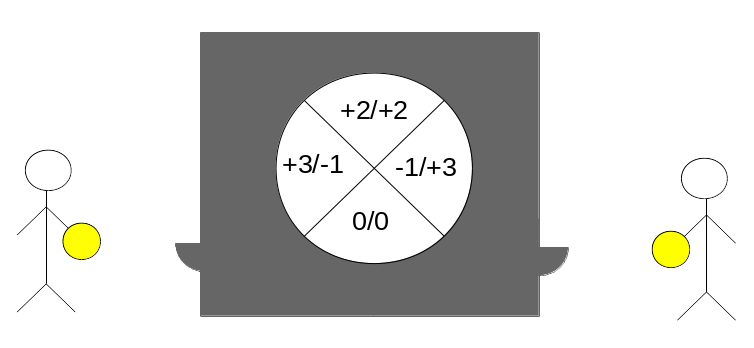
\includegraphics[scale=0.5]{coin_game.png}\\
Left corner $\rightarrow$ (1) cheats and (2) cooperates\\
Right corner $\rightarrow$ (1) cooperates and (2) cheats\\
Top corner $\rightarrow$ both cooperate\\
Bottom corner $\rightarrow$ both cheat\\
\end{center}
Let us consider a sequential variant of the prisoner's dilemma. A quick reminder would be to tell that two prisoners can cooperate or snitch each other, without knowing in advance the other's move.

Here, the two players have the choice to put a coin (cooperate) or not (cheat) during $N$ trials. Each player seeks to collect the most number of coins. A negative value can be seen as a debt. Also, there is a probability $p$ for a player to make a mistake, i.e. pick the non chosen move.

Let's start with $N = 10$.

\begin{itemize}
	\item Draw the game tree using probability $p$. Which search algorithm should you use in which case ?
	\item Try with $p = 0,0.25,0.5,0.75$, using . What can you tell ? If you feel that $N$ is too small to see something, feel free to increase it. If $N$ is too large, use your computer to simulate.  
\end{itemize}








%\begin{description}
%	\item[empty] ist der Seitenstil, bei dem Kopf- und Fusszeile vollständig 	leer bleiben.\marginpar[\textit{Randnotiz links}]
%	{\textit{Randnotiz rechts}}
%    \item[plain] ist der Seitenstil, bei dem keinerlei Kolumnentitel verwendet wird.
%    \item[headings] ist der Seitenstil für automatische Kolumnentitel.
%    \item[myheadings] ist der Seitenstil für manuelle Kolumnentitel.
%\end{description}



%$\mathsf{({m}^{3}/s)}$
%-------------------------------
%\begin{figure}
%	\setcapindent{-1em}
%    \fbox{\parbox{.95\linewidth}{
%    	\centering\KOMAScript}}
%	\caption{Beispiel mit teilweise hängendem Einzug ab der zweiten Zeile}
%\end{figure}

%Guten Morgen\footnote{irgend ein text\label{refnote}}\multiplefootnoteseparator\footnote{es geht noch weiter}Blabla\footref{refnote}
\end{document}
